\section{Introduction}

In this section we will tour some phenomena concerning the loci of triangle centers over elliptic billard 3-periodics, including the loci of vertices of certain derived triangles.

Recall the loci of the incenter $X_1$ and excenters (vertices of the excentral family) were previously shown to be ellipses, see \cref{sec:03-inc-exc-loci} and \cref{fig:billiard-grid}. Recall also that the locus of the Mittenpunkt $X_9$ is a point, see \cref{sec:03-stationary}.

\begin{itemize}
\item confocal
    \begin{itemize}
        \item loci of incenter, excenters
        \item loci of intouchpoints
        \item loci od X1,X2,X3,X4,X5
        \item loci of X11 and X100
        \item loci of derived triangle vertices: extouch (caustic), intouch (sextic), feuerbach triangle, medial, anticomplementary 
    \end{itemize}
    \item brocard points
\end{itemize}

We will omit most proofs etc.

\section{Loci of the first five Kimberling centers}

The semi-axes $a_1,b_1$ for the elliptic locus of the incenter $X_1$ were given in \cref{thm:03-incenter-excenter}. It turns the loci of the next four centers in \cite{etc} are also ellipses. There are the barycenter $X_2$, the circumcenter $X_3$, the orthocenter $X_4$, and the center of the 9-point circle (also known as Euler's circle) $X_5$. Their semi-axes are given by:

\begin{align*}
    \left(a_2,b_2\right)=&k_2\left(a,b\right),\;\text{with}\; k_2=\frac{2\delta -a^{2}-b^{2}}{3c^2}\\
     \left(a_3,b_3\right)=&\left(\frac{a^{2}-\delta}{2a},\frac{\delta-b^{2}}{2b}\right)\\
 \left(a_4,b_4\right)=&\left(\frac{k_4}a,\frac{k_4}b\right),\;\text{with}\;k_4=\frac{  (a^{2}+b^{2})\delta-2\,a^{2}b^{2} }{c^2}\\
   \left(a_5,b_5\right)=&\left(\frac{- w'_5(a,b)+ w''_5(a,b) \delta}{ w_5(a,b)},\;\frac{ w'_5(b,a)-{w''_5(b,a) \delta}}{w_5(b,a)}\right)
\end{align*}
where $w'_5(u,v)=u^2(u^2+3v^2)$, $w''_5(u,v)=3u^2+ v^2$, and $w_5(u,v)=4u(u^2-v^2)$. Note that (i) $a_2/b_2=a/b$ and (ii) $b_4/a_4=a/b$.

As it turns out, the locus of 49 out of the first 200 centers in \cite{etc} are ellipses. These are: $X_k$, $k=$1,  2,  3,  4,  5,  7,  8,  10,  11,  12,  20,  21,  35,  36,  40,  46,  55,  56,  57,  63,  65,  72,  78,  79,  80,  84,  88,  90,  100,  104,  119,  140,  142,  144,  145,  149,  153,  162,  165,  190,  191,  200. Links to live animations as well as expressions for their semi-axes are provided in \cite{garcia2021-ellipses-web}.

%% Swans
%% the following centers lie on the $X_9$-centered circumellipse: 88, 100, 162, 190 \cite{etc}.

\begin{figure}
\centering
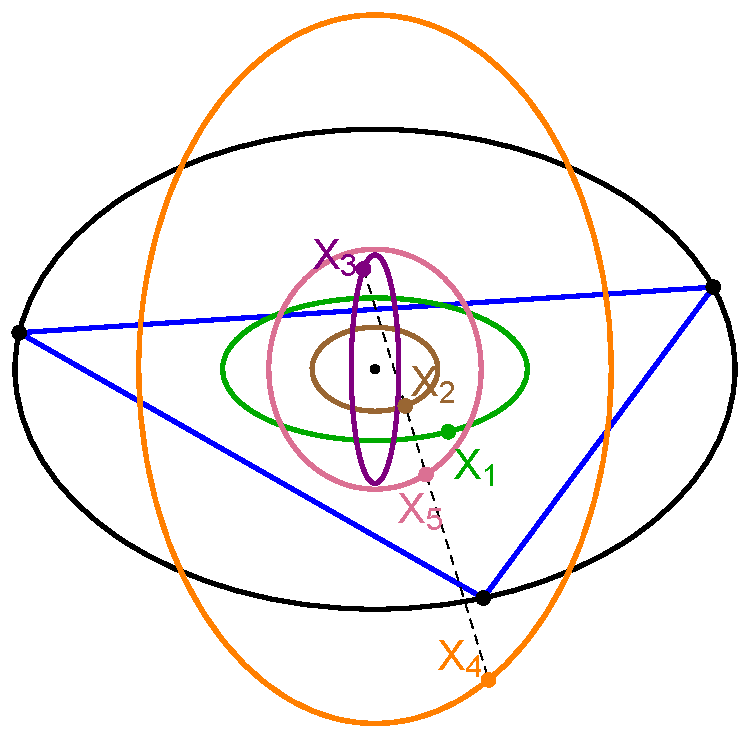
\includegraphics[width=.6\textwidth]{pics_04_060_locus_x12345.pdf}
\caption{Over billiard 3-periodics, the loci of incenter $X_1$, barycenter $X_2$, circumcenter $X_3$, orthocenter $X_4$, and 9-point center $X_5$ are all ellipses. The Euler line (dashed black) is shown passing through all but the first center. \href{https://youtu.be/sMcNzcYaqtg}{Video}, \href{https://bit.ly/3eVScgE}{Live}}
\label{fig:04-x12345}
\end{figure}

%%% begin X4
\section{The locus of the orthocenter: when 3-periodics are obtuse}

\begin{figure}
    \centering
    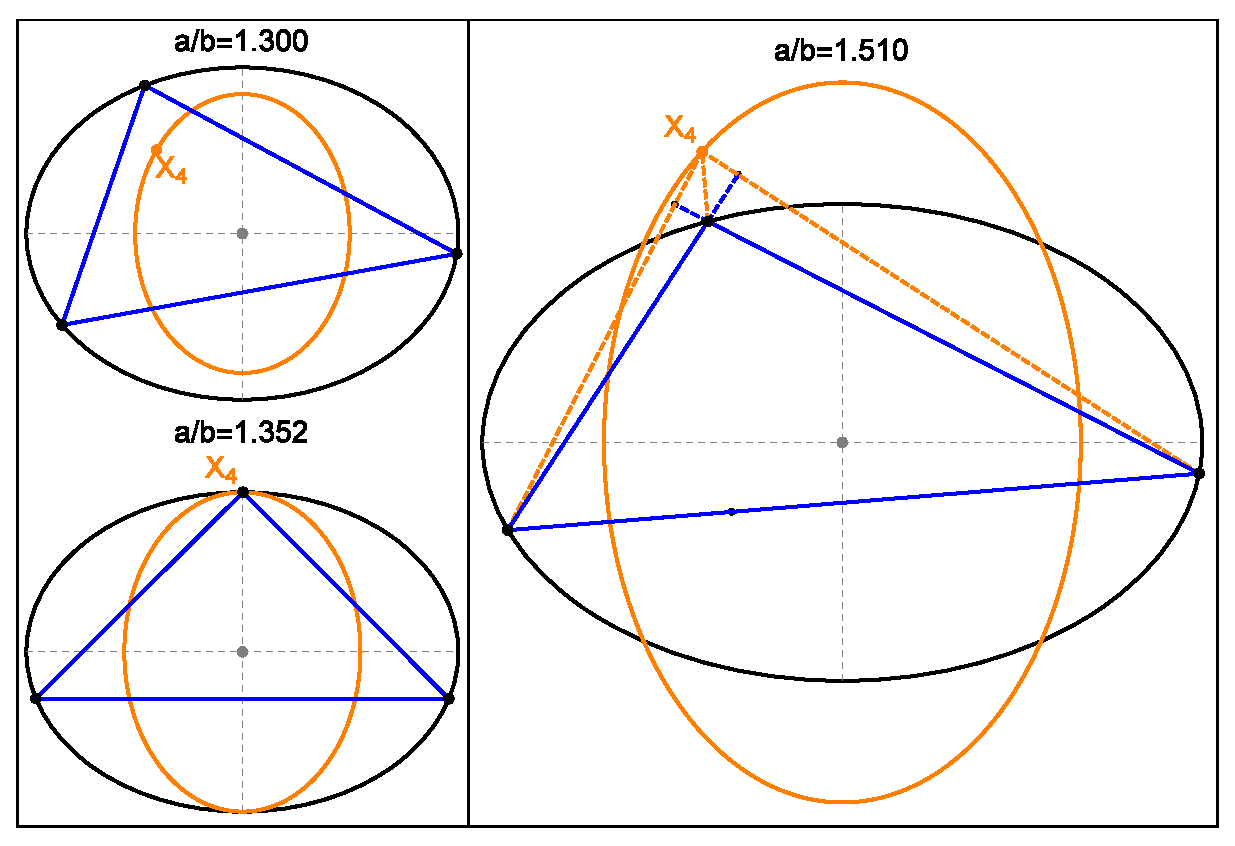
\includegraphics[width=\textwidth]{pics_04_130_ort_loci.eps}
    \caption{Locus of the orthocenter (orange) over elliptic billiards with different aspect ratios. If $a/b$ is (i) less than (resp. (ii) equal, (iii) greater than) $\alpha_4{\simeq}1.352$, the locus of the orthocenter $X_4$ (orange) is (i) interior (resp. (ii) internally tangent, (iii) intersecting) with the elliptic billiard. In (i) and (ii) all 3-periodics are acute, whereas in (iii) some will be obtuse.}.
    \label{fig:04-orthocenter-loci}
\end{figure}

It turns out the locus of $X_4$ can be used to determine if the billiard 3-period family will contain obtuse triangles. Referring to Figure~\ref{fig:04-orthocenter-loci}:

\begin{proposition}
The locus of $X_4$ is internally tangent to the elliptic billiard at its top and bottom vertices when $a/b=\alpha_4$ given by:

\[\sqrt{2\,\sqrt {2}-1}\;{\simeq}\;1.352.\]
\end{proposition}

\begin{proof}
The equation $b_4=b$ is equivalent to $a^4+2a^2b^2-7b^4=0.$ Therefore, as $a>b>0$, it follows that $a/b=\sqrt{2\,\sqrt {2}-1}.$
\end{proof}

\noindent Let $\alpha_4^*$ be the positive root of
${x}^{6}+{x}^{4}-4\,{x}^{3}-{x}^{2}-1=0$, i.e.,
$\alpha_4^{*}={\simeq}\;1.51$. 

\begin{proposition}
When $a/b=\alpha_4^{*}$, then $a_4=b$ and $b_4=a$, i.e., the locus of $X_4$ is identical to a rotated copy of Billiard. 
\end{proposition}

\begin{proof}
The condition $a_4=b$, or equivalently $b_4=a$, is defined by $a^6+a^4b^2-4a^3b^3-a^2b^4-b^6=0$. Graphic analysis shows that ${x}^{6}+{x}^{4}-4\,{x}^{3}-{x}^{2}-1=0$ has only one positive real root which we call $\alpha_4^*$.
\end{proof}

\begin{theorem}
If $a/b<\alpha_4$ (resp. $a/b>\alpha_4$) the 3-periodic family will not (resp. will) contain obtuse triangles.
\end{theorem}

\begin{proof}
If the 3-periodic is acute, $X_4$ is in its interior, therefore also internal to the EB. If the 3-periodic is a right triangle, $X_4$ lies on the right-angle vertex and is therefore on the EB. If the 3-periodic is obtuse, $X_4$ lies on exterior wedge between sides incident on the obtuse vertex (feet of altitudes are exterior). Since the latter is on the EB, $X_4$ is exterior to the EB.
\end{proof}
%%% end X4

%%% begin X6
\section{Quartic locus of the symmedian point \torp{$X_6$}{X(6)}}
\label{sec:symmedian}

The symmedian point $X_6$ is replete with properties, indeed it is known as the crown jewel of triangle geometry \cite[Symmedian Point]{mw}. Its construction is deceptively simple: the point where a triangle's {\em symmedians} concur; these are reflections of medians on the bisectors. Its trilinear coordinates could not be simpler: $[a:b:c]$. However, it is the first Kimberling center whose locus over billiard 3-periodics is {\em not} an ellipse. 

In fact, when $1<a/b<2$, its locus is visually indistinguishable from a true ellipse; see Figure~\ref{fig:04-locus-x6}. Fortunately, its fit error is easily detectable with numerical methods. Indeed:

\begin{proposition}
The locus of $X_6$ is a convex quartic given by:

\begin{equation*}
  \X_6(x,y)=c_1 x^4+c_2 y^4+c_3 x^2 y^2+ c_4 x^2 + c_5 y^2 = 0
\end{equation*}

\noindent where:
$$
\begin{array}{rlrl}
c_1=&b^4(5\delta^2-4(a^2-b^2)\delta -a^2 b^2)&c_2=&a^4(5\delta^2+4(a^2-b^2)\delta-a^2b^2) \\
c_3=&2a^2 b^2(a^2 b^2+3\delta^2)&c_4=&a^2 b^4(3 b^4+2(2 a^2-b^2)\delta-5\delta^2)\\
c_5=&a^4 b^2(3 a^4+2(2 b^2-a^2)\delta-5\delta^2)&\delta=&\sqrt{a^4-a^2 b^2+b^4}
\end{array}
$$
\end{proposition}

\begin{proof}
Using a CAS, obtain symbolic expressions for the coefficients of a quartic symmetric about both axes (no odd-degree terms), passing through 5 known-points. Still using a CAS, verify the symbolic parametric for the locus satisfies the quartic.
\end{proof}

 \noindent Note the above is also satisfied by a degenerate level curve $(x,y)=(0,0)$, which we ignore.

\begin{remark}
We term the ``best-fit'' ellipse $\mathcal{E}_6$ the one internally-tangent to $\X_6(x,y)=0$ at its four vertices. Its semi-axes are given by: 

{\small  
\begin{align*}
%a_6=&\frac{\left[(3\,a^2-b^2)\delta %-(a^2+b^2)b^2\right]a}{a^4+b^4+2\delta^2}\nonumber\\
a_6= \frac{\left[(3\,a^2-b^2)\delta -(a^2+b^2)b^2\right]a}{a^2b^2+3\delta^2},\;\;\;
b_6= \frac{\left[(a^2-3\,b^2)\delta + (a^2+b^2)a^2\right]b}{a^2b^2+3\delta^2}
\label{eqn:x6-ellipse}
\end{align*}
}
\end{remark}

Table~\ref{tab:quartic-coeffs} shows the above coefficients numerically for a few values of $a/b$.

\begin{table}
    \centering
$$
\begin{array}{|c|c|c|c|c|c|c|c|}
\hline
 \text{a/b} & a_6 & b_6 & c_1/c_3 & c_2/c_3 & c_4/c_3 & c_5/c_3 & A(\mathcal{E}_6)/A(\mathcal{X}_6) \\
 \hline
  1.25 & 0.433 & 0.282 & 0.211 & 1.185 & -0.040 & -0.095 & 0.9999 \\
 1.50 & 0.874 & 0.427 & 0.114 & 2.184 & -0.087 & -0.399 & 0.9998 \\
 2.00 & 1.612 & 0.549 & 0.052 & 4.850 & -0.134 & -1.461 & 0.9983 \\
 3.00 & 2.791 & 0.620 & 0.020 & 12.423 & -0.157 & -4.769 & 0.9949 \\
 \hline
\end{array}
$$
\caption{Coefficients $c_i/c_3$, $i=1,2,4,5$ for the quartic locus of $X_6$ as well as the axes $a_6,b_6$ for the best-fit ellipse, for various values of $a/b$. The last-column reports the area ratio of the internal ellipse $\mathcal{E}_6$ (with axes $a_6,b_6$) to that of the quartic locus $\mathcal{X}_6$, showing an almost exact match.}
\label{tab:quartic-coeffs}
\end{table}


\begin{figure}
    \centering
    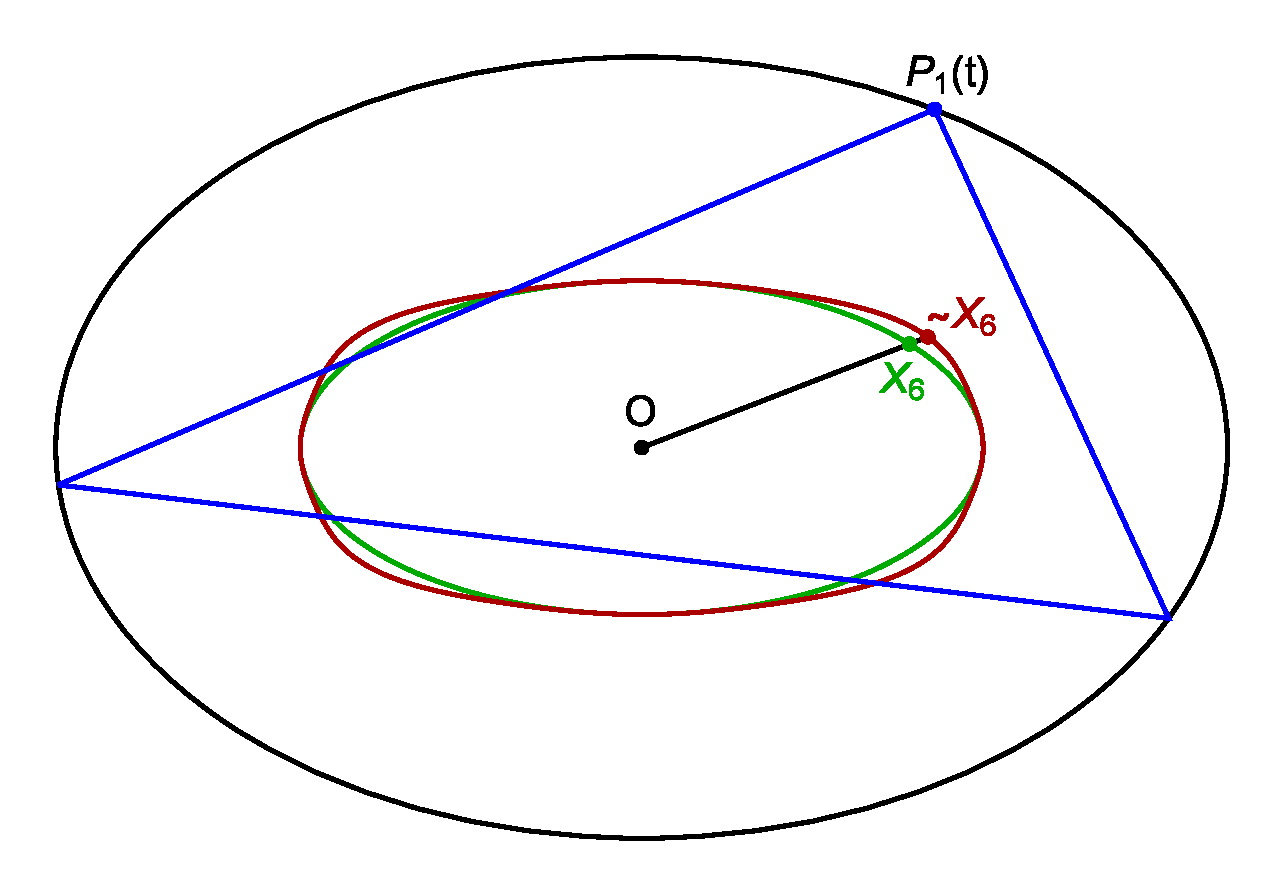
\includegraphics[width=.7\textwidth]{pics_04_090_symmedian.eps}
    \caption{Over billiard 3-periodics (blue), the locus of the symmedian point $X_6$ is a quartic (green). At the billiard aspect ratio shown, it is visually identical to an ellipse. Also shown is a copy of the quartic (red) such that the distance to a best-fit ellipse (green) is scaled 1000 fold. \href{https://bit.ly/3hxOZoV}{Live}}
    \label{fig:04-locus-x6}
\end{figure}
%%% end X6

%%% BEGIN X11 and X100
\begin{figure}
    \centering
    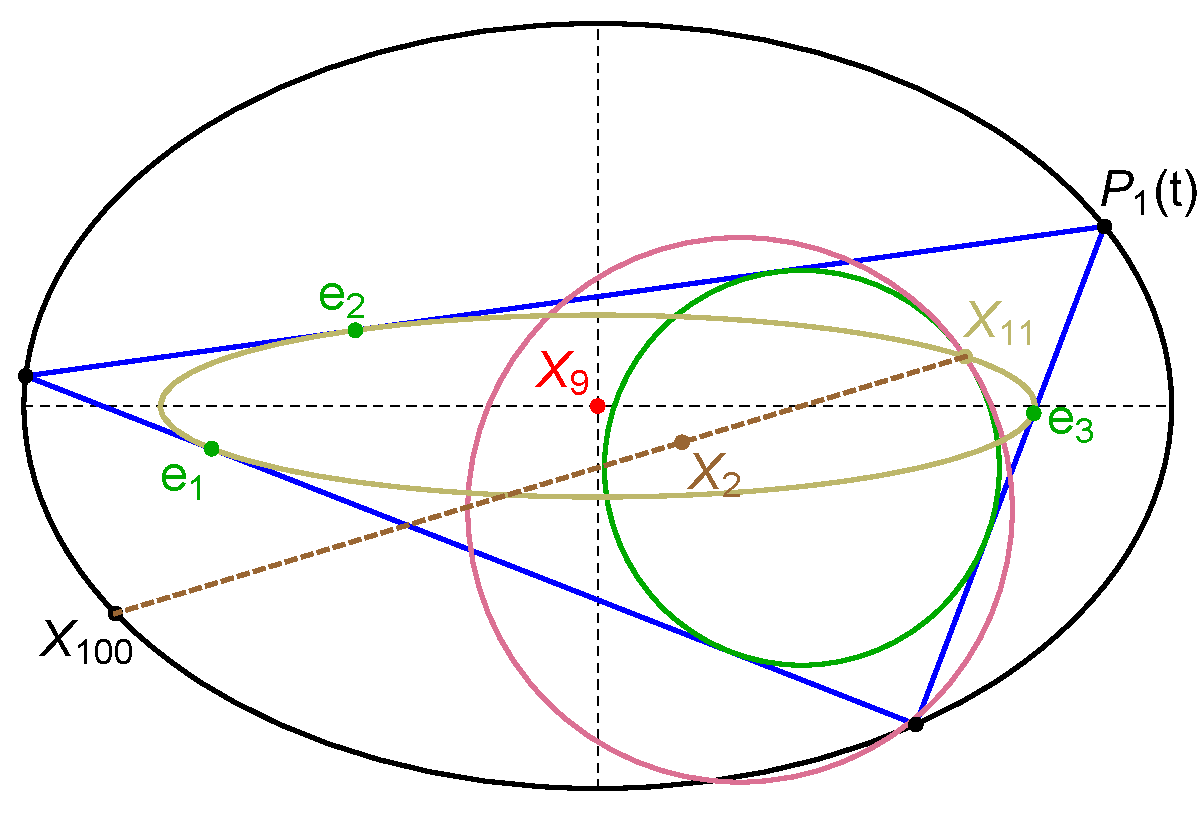
\includegraphics[width=.7\textwidth]{pics_04_080_feuerbach_loci.pdf}
    \caption{A billiard 3-periodic (blue). Also shown are the incircle (green) and 9-point circle (pink) which touch at the Feuerbach point $X_{11}$. Also shown is the latter's {\em anticomplement} $X_{100}$, and the three extouchpoints $e_1,e_2,e_3$. Over the billiard family, $X_{100}$ sweep the billiard while both $X_{11}$ and the extouchpoints sweep the caustic (though in opposite directions).
    % done
    \href{https://youtu.be/TXdg7tUl8lc}{Video},
    \label{fig:04-feuer-loci} \href{https://bit.ly/2S2LVqp}{Live}}
\end{figure}

\section{The locus of the Feuerbach point and its anticomplement}

Referring to \cref{fig:04-locus-x11-x100}, the Feuerbach point $X_{11}$ is the single point of contact between incircle and 9-point circle \cite[X(11)]{mw}. $X_{11}$ is known to lie on the $X_{9}$-centered inconic, i.e., the  Mandart inellipse \cite[Mandart inellipse]{mw}. Since the latter is unique:

\begin{observation}
The confocal caustic is the stationary Mandart inellipse of billiard 3-periodics.
\end{observation}

Therefore:

\begin{proposition}
Over billiard 3-periodics, $X_{11}$ sweepts the confocal caustic.
\end{proposition}

The anticomplement of a point $P$ is its double-length reflection about the barycenter $X_2$, i.e., $A(P) = X_2+2 X_2-P$. Stille referring,  \cref{fig:04-locus-x11-x100}, $X_{100}$ is the anticomplement of $X_{11}$. This point is known to lie on (i) the circumcircle, (ii) the Steiner circumellipse (centered on $X_2$), and most relevantly here, (iii) on the $X_9$-centered circumellipse \cite[X(9)]{etc}. Since the latter is unique:

\begin{observation}
The elliptic billiard is the stationary $X_9$-centered circumconic of billiard 3-periodics.
\end{observation}

Therefore:

\begin{proposition}
Over billiard 3-periodics, the locus of $X_{100}$ is the elliptic billiard.
\end{proposition}

The vertices of the so-called {\em extouch triangle} are the points of contact of the excircles with a triangle's sidelines \cite[Extouch triangle]{mw}. These are also known as {\em extouchpoints}. A known fact is that the Mandart inellipse (i.e., the caustic) touches a triangle's sidelines at the extouchpoints \cite[Mandart inellipse]{mw}. Therefore:

\begin{proposition}
Over billiard 3-periodics, the locus of the extouchpoints is the confocal caustic.
\end{proposition}

This is also illustrated in \cref{fig:04-locus-x11-x100}. A curious dynamic phenomenon is that while the extouchpoints follow the direction of motion of billiard 3-periodics along the outer ellipse (e.g., counter- or clockwise), $X_{11}$ rotates in the opposite direction; see this \href{https://bit.ly/2S2LVqp}{Live}.


%%% END X11 and X100

\section{Locus of vertices of some derived triangles}

A few triangles derived from billiard 3-periodics are shown in \cref{fig:04-derived-isosceles}. For their definitions see \cite{app:app-triangle} and \cite{mw}.

\begin{figure}
    \centering
    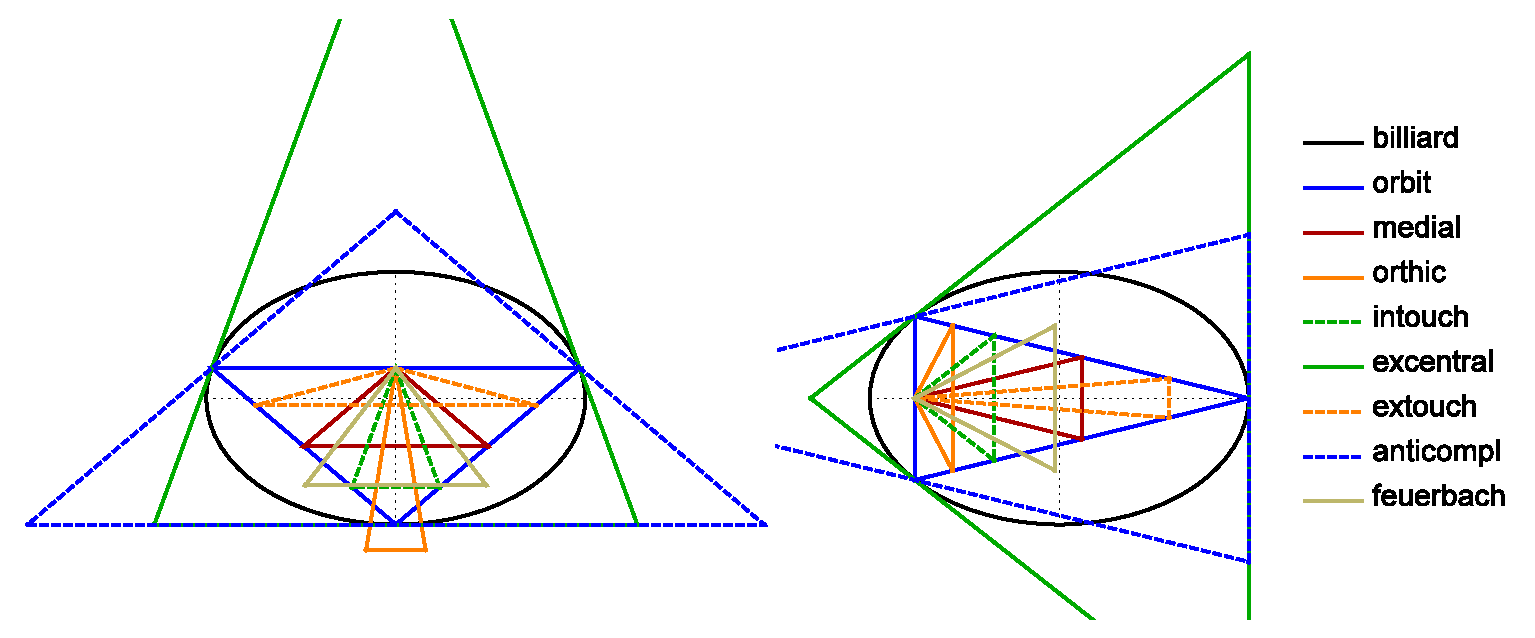
\includegraphics[width=\textwidth]{pics_04_100_confocal_derived.eps}
    \caption{Triangles derived from an isosceles billiard 3-periodic (blue). These contain one vertex on the axis of symmetry. \href{https://youtu.be/xyroRTEVNDc}{Video}}
    \label{fig:04-derived-isosceles}
\end{figure}

Mentioned in \cref{sec:01-introduction} was an early experiment which showed that over billiard 3-periodics, the locus of the vertices of the intouch triangle (i.e., the intouchpoints) is a 2-lobed, self-intersect curve; see \cref{fig:01-intouch-x59}.

As shown in \cref{fig:04-locus-x11-x100}, the loci of vertices of some other triangles derived from billiard 3-periodics aren't ellipses. A noteworthy exception is the extouch triangle, mentioned above.

\begin{figure}
    \centering
    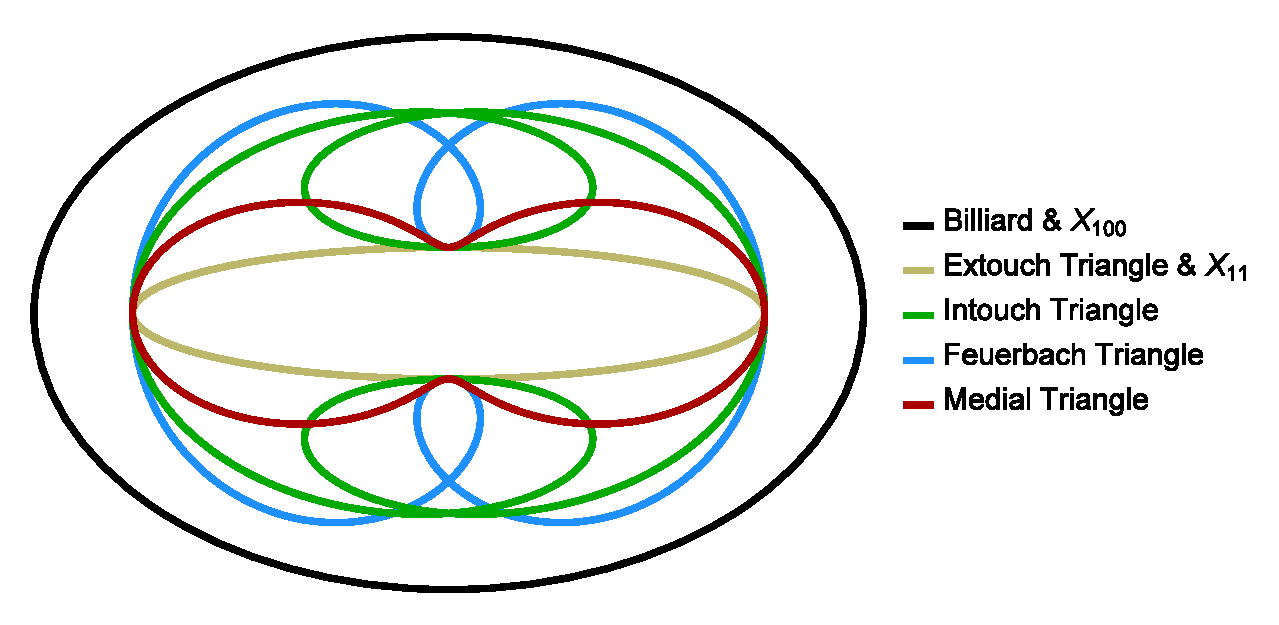
\includegraphics[width=\textwidth]{pics_04_070_non_elliptic.eps}
    \caption{Over billiard 3-periodics, the loci of vertices of certain derived triangles is non-elliptic, namely: the (i) intouch (green), (ii) Feuerbach (not to be confused with the Feuerbach {\em point}) (blue), (iii) medial (red), triangles, and many others not shown. A noteworthy excpetion is the extouch triangle, whose vertices sweep the confocal caustic.
     \href{https://youtu.be/OGvCQbYqJyI}{Video}}
    \label{fig:04-locus-x11-x100}
\end{figure}

% \includegraphics[trim={left bot right upper},clip]
\begin{figure}
    \centering
    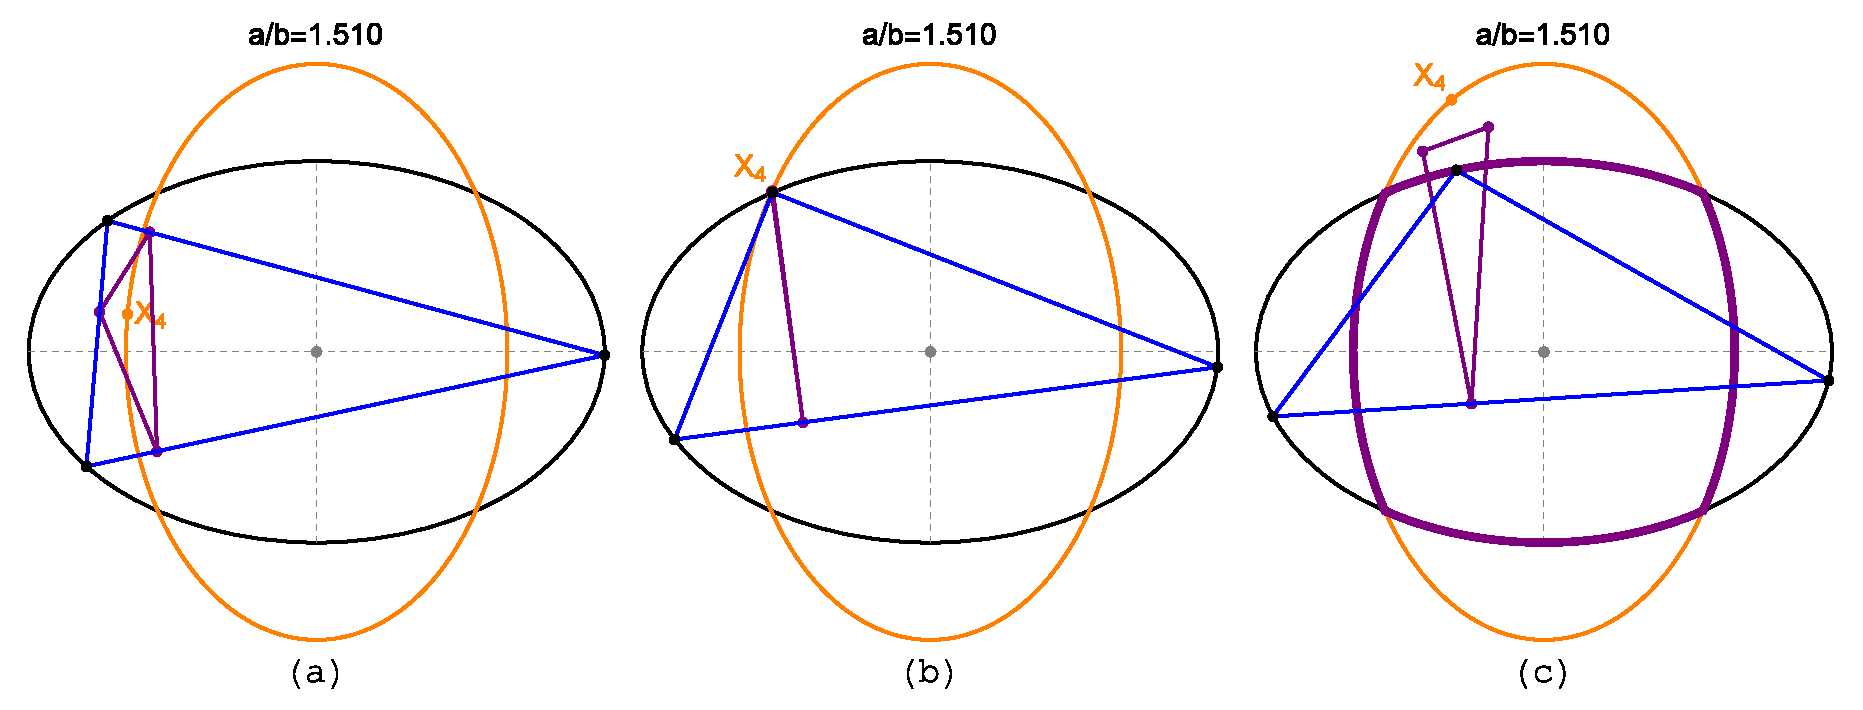
\includegraphics[trim={0 0 0 20},clip,width=\textwidth]{pics_04_120_ort_loci_kink.eps}
    \caption{Let $T$ and $T_h$ be a billiard 3-periodic and its Orthic Triangle (blue and purple, respectively). Above (resp. below) a certain aspect ratio, the locus of the incenter of the orthic is a 4-elliptic arc quadrilateral (resp. ellipse). Shown here are 3 snapshots of the former case. \textbf{(a)} $T$ is acute ($X_4$ is interior to the EB), and $I_h=X_4$. \textbf{(b)} $X_4$ is on the EB and $T$ is a right triangle. $T_h$ degenerates to a segment. \textbf{(c)} $X_4$ is exterior to the EB. Two of $T_h$'s vertices are outside $T$. $I_h$ is pinned to $T$'s obtuse vertex, on the EB. $X_4$ is an Excenter of the 3-periodic. The complete locus of $I_h$ comprises therefore 4 elliptic arcs (thick purple) joined at the corners. \href{https://youtu.be/3qJnwpFkUFQ}{Video}, \href{https://bit.ly/33TVjit}{Live}}
    \label{fig:orthic_incenter_locus}
\end{figure}

%%% BEGIN EXERCISES
\section{Exercises}

\begin{exercise}
Calculate the elliptic billiard aspect ratio $a/b$ such that top and bottom vertices of the elliptic locus of $X_3$ coincide each with the billiard top and bottom vertices. Repeat for the locus of $X_5$.
\end{exercise}

\begin{exercise}
Calculate the elliptic billiard aspect ration $a/b$ such that the locus of $X_4$ is identical to a $90^\circ$ rotated copy of billiard.
\end{exercise}

\begin{exercise}
Over billiard 3-periodics, the envelope of the Euler line is an astroidal-like curve with four cusps, see it \href{https://bit.ly/3yiCvrn}{Live}. Derive its equation. Also, find the elliptic billiard aspect ratio $a/b$ such that the top and bottom cusps of said curve coincide each with top and bottom vertices of the elliptic billiard.
\end{exercise}